% Created by tikzDevice version 0.7.0 on 2014-07-24 03:38:00
% !TEX encoding = UTF-8 Unicode
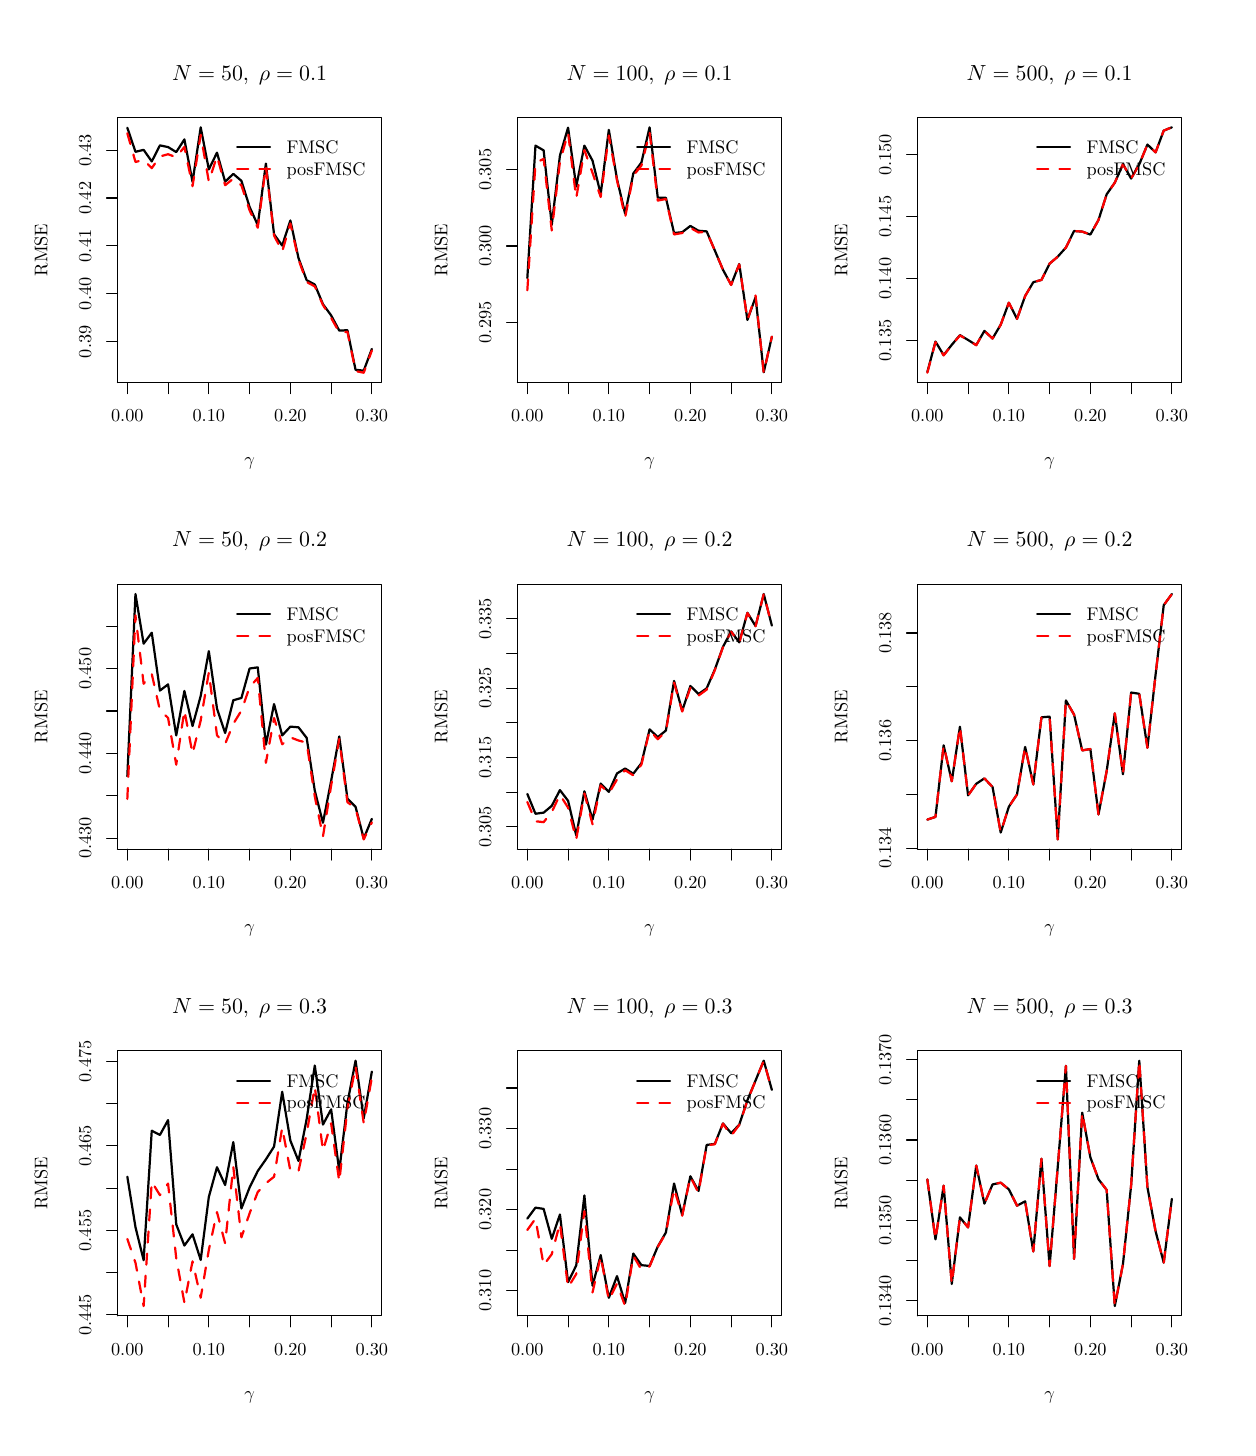
\begin{tikzpicture}[x=1pt,y=1pt]
\definecolor[named]{fillColor}{rgb}{1.00,1.00,1.00}
\path[use as bounding box,fill=fillColor,fill opacity=0.00] (0,0) rectangle (433.62,505.89);
\begin{scope}
\path[clip] ( 32.47,377.65) rectangle (127.91,473.42);
\definecolor[named]{drawColor}{rgb}{0.00,0.00,0.00}

\path[draw=drawColor,line width= 0.8pt,line join=round,line cap=round] ( 36.01,469.71) --
	( 38.95,461.03) --
	( 41.90,461.73) --
	( 44.84,457.55) --
	( 47.79,463.35) --
	( 50.73,462.74) --
	( 53.68,460.93) --
	( 56.63,465.50) --
	( 59.57,450.16) --
	( 62.52,469.87) --
	( 65.46,454.66) --
	( 68.41,460.73) --
	( 71.35,450.21) --
	( 74.30,453.06) --
	( 77.24,450.53) --
	( 80.19,441.11) --
	( 83.14,434.55) --
	( 86.08,456.78) --
	( 89.03,431.20) --
	( 91.97,427.15) --
	( 94.92,436.21) --
	( 97.86,422.64) --
	(100.81,414.64) --
	(103.75,413.07) --
	(106.70,405.97) --
	(109.65,401.93) --
	(112.59,396.42) --
	(115.54,396.56) --
	(118.48,382.26) --
	(121.43,381.95) --
	(124.37,389.80);
\end{scope}
\begin{scope}
\path[clip] (  0.00,  0.00) rectangle (433.62,505.89);
\definecolor[named]{drawColor}{rgb}{0.00,0.00,0.00}

\path[draw=drawColor,line width= 0.4pt,line join=round,line cap=round] ( 36.01,377.65) -- (124.37,377.65);

\path[draw=drawColor,line width= 0.4pt,line join=round,line cap=round] ( 36.01,377.65) -- ( 36.01,373.69);

\path[draw=drawColor,line width= 0.4pt,line join=round,line cap=round] ( 50.73,377.65) -- ( 50.73,373.69);

\path[draw=drawColor,line width= 0.4pt,line join=round,line cap=round] ( 65.46,377.65) -- ( 65.46,373.69);

\path[draw=drawColor,line width= 0.4pt,line join=round,line cap=round] ( 80.19,377.65) -- ( 80.19,373.69);

\path[draw=drawColor,line width= 0.4pt,line join=round,line cap=round] ( 94.92,377.65) -- ( 94.92,373.69);

\path[draw=drawColor,line width= 0.4pt,line join=round,line cap=round] (109.65,377.65) -- (109.65,373.69);

\path[draw=drawColor,line width= 0.4pt,line join=round,line cap=round] (124.37,377.65) -- (124.37,373.69);

\node[text=drawColor,anchor=base,inner sep=0pt, outer sep=0pt, scale=  0.66] at ( 36.01,363.40) {0.00};

\node[text=drawColor,anchor=base,inner sep=0pt, outer sep=0pt, scale=  0.66] at ( 65.46,363.40) {0.10};

\node[text=drawColor,anchor=base,inner sep=0pt, outer sep=0pt, scale=  0.66] at ( 94.92,363.40) {0.20};

\node[text=drawColor,anchor=base,inner sep=0pt, outer sep=0pt, scale=  0.66] at (124.37,363.40) {0.30};

\path[draw=drawColor,line width= 0.4pt,line join=round,line cap=round] ( 32.47,392.39) -- ( 32.47,461.65);

\path[draw=drawColor,line width= 0.4pt,line join=round,line cap=round] ( 32.47,392.39) -- ( 28.51,392.39);

\path[draw=drawColor,line width= 0.4pt,line join=round,line cap=round] ( 32.47,409.70) -- ( 28.51,409.70);

\path[draw=drawColor,line width= 0.4pt,line join=round,line cap=round] ( 32.47,427.02) -- ( 28.51,427.02);

\path[draw=drawColor,line width= 0.4pt,line join=round,line cap=round] ( 32.47,444.33) -- ( 28.51,444.33);

\path[draw=drawColor,line width= 0.4pt,line join=round,line cap=round] ( 32.47,461.65) -- ( 28.51,461.65);

\node[text=drawColor,rotate= 90.00,anchor=base,inner sep=0pt, outer sep=0pt, scale=  0.66] at ( 22.97,392.39) {0.39};

\node[text=drawColor,rotate= 90.00,anchor=base,inner sep=0pt, outer sep=0pt, scale=  0.66] at ( 22.97,409.70) {0.40};

\node[text=drawColor,rotate= 90.00,anchor=base,inner sep=0pt, outer sep=0pt, scale=  0.66] at ( 22.97,427.02) {0.41};

\node[text=drawColor,rotate= 90.00,anchor=base,inner sep=0pt, outer sep=0pt, scale=  0.66] at ( 22.97,444.33) {0.42};

\node[text=drawColor,rotate= 90.00,anchor=base,inner sep=0pt, outer sep=0pt, scale=  0.66] at ( 22.97,461.65) {0.43};

\path[draw=drawColor,line width= 0.4pt,line join=round,line cap=round] ( 32.47,377.65) --
	(127.91,377.65) --
	(127.91,473.42) --
	( 32.47,473.42) --
	( 32.47,377.65);
\end{scope}
\begin{scope}
\path[clip] (  0.00,337.26) rectangle (144.54,505.89);
\definecolor[named]{drawColor}{rgb}{0.00,0.00,0.00}

\node[text=drawColor,anchor=base,inner sep=0pt, outer sep=0pt, scale=  0.79] at ( 80.19,486.92) {\bfseries $N=50, \;\rho=0.1$};

\node[text=drawColor,anchor=base,inner sep=0pt, outer sep=0pt, scale=  0.66] at ( 80.19,347.56) {$\gamma$};

\node[text=drawColor,rotate= 90.00,anchor=base,inner sep=0pt, outer sep=0pt, scale=  0.66] at (  7.13,425.53) {RMSE};
\end{scope}
\begin{scope}
\path[clip] ( 32.47,377.65) rectangle (127.91,473.42);
\definecolor[named]{drawColor}{rgb}{1.00,0.00,0.00}

\path[draw=drawColor,line width= 0.8pt,dash pattern=on 4pt off 4pt ,line join=round,line cap=round] ( 36.01,467.73) --
	( 38.95,457.36) --
	( 41.90,458.09) --
	( 44.84,455.12) --
	( 47.79,459.35) --
	( 50.73,460.15) --
	( 53.68,459.08) --
	( 56.63,462.79) --
	( 59.57,448.60) --
	( 62.52,467.17) --
	( 65.46,450.28) --
	( 68.41,459.43) --
	( 71.35,448.95) --
	( 74.30,451.33) --
	( 77.24,448.89) --
	( 80.19,439.87) --
	( 83.14,433.59) --
	( 86.08,455.77) --
	( 89.03,430.80) --
	( 91.97,424.99) --
	( 94.92,435.14) --
	( 97.86,422.12) --
	(100.81,413.98) --
	(103.75,412.39) --
	(106.70,405.67) --
	(109.65,401.04) --
	(112.59,395.80) --
	(115.54,395.99) --
	(118.48,381.80) --
	(121.43,381.20) --
	(124.37,389.23);
\definecolor[named]{drawColor}{rgb}{0.00,0.00,0.00}

\path[draw=drawColor,line width= 0.8pt,line join=round,line cap=round] ( 75.72,462.63) -- ( 87.60,462.63);
\definecolor[named]{drawColor}{rgb}{1.00,0.00,0.00}

\path[draw=drawColor,line width= 0.8pt,dash pattern=on 4pt off 4pt ,line join=round,line cap=round] ( 75.72,454.71) -- ( 87.60,454.71);
\definecolor[named]{drawColor}{rgb}{0.00,0.00,0.00}

\node[text=drawColor,anchor=base west,inner sep=0pt, outer sep=0pt, scale=  0.66] at ( 93.54,460.35) {FMSC};

\node[text=drawColor,anchor=base west,inner sep=0pt, outer sep=0pt, scale=  0.66] at ( 93.54,452.43) {posFMSC};
\end{scope}
\begin{scope}
\path[clip] (177.01,377.65) rectangle (272.45,473.42);
\definecolor[named]{drawColor}{rgb}{0.00,0.00,0.00}

\path[draw=drawColor,line width= 0.8pt,line join=round,line cap=round] (180.55,415.39) --
	(183.49,463.26) --
	(186.44,461.55) --
	(189.38,434.64) --
	(192.33,459.67) --
	(195.27,469.77) --
	(198.22,448.48) --
	(201.17,463.26) --
	(204.11,457.83) --
	(207.06,445.75) --
	(210.00,468.96) --
	(212.95,451.16) --
	(215.89,438.66) --
	(218.84,453.18) --
	(221.78,457.17) --
	(224.73,469.87) --
	(227.68,444.49) --
	(230.62,444.40) --
	(233.57,431.69) --
	(236.51,431.98) --
	(239.46,434.24) --
	(242.40,432.51) --
	(245.35,432.27) --
	(248.29,425.40) --
	(251.24,418.40) --
	(254.19,412.99) --
	(257.13,420.47) --
	(260.08,400.27) --
	(263.02,408.50) --
	(265.97,381.36) --
	(268.91,394.19);
\end{scope}
\begin{scope}
\path[clip] (  0.00,  0.00) rectangle (433.62,505.89);
\definecolor[named]{drawColor}{rgb}{0.00,0.00,0.00}

\path[draw=drawColor,line width= 0.4pt,line join=round,line cap=round] (180.55,377.65) -- (268.91,377.65);

\path[draw=drawColor,line width= 0.4pt,line join=round,line cap=round] (180.55,377.65) -- (180.55,373.69);

\path[draw=drawColor,line width= 0.4pt,line join=round,line cap=round] (195.27,377.65) -- (195.27,373.69);

\path[draw=drawColor,line width= 0.4pt,line join=round,line cap=round] (210.00,377.65) -- (210.00,373.69);

\path[draw=drawColor,line width= 0.4pt,line join=round,line cap=round] (224.73,377.65) -- (224.73,373.69);

\path[draw=drawColor,line width= 0.4pt,line join=round,line cap=round] (239.46,377.65) -- (239.46,373.69);

\path[draw=drawColor,line width= 0.4pt,line join=round,line cap=round] (254.19,377.65) -- (254.19,373.69);

\path[draw=drawColor,line width= 0.4pt,line join=round,line cap=round] (268.91,377.65) -- (268.91,373.69);

\node[text=drawColor,anchor=base,inner sep=0pt, outer sep=0pt, scale=  0.66] at (180.55,363.40) {0.00};

\node[text=drawColor,anchor=base,inner sep=0pt, outer sep=0pt, scale=  0.66] at (210.00,363.40) {0.10};

\node[text=drawColor,anchor=base,inner sep=0pt, outer sep=0pt, scale=  0.66] at (239.46,363.40) {0.20};

\node[text=drawColor,anchor=base,inner sep=0pt, outer sep=0pt, scale=  0.66] at (268.91,363.40) {0.30};

\path[draw=drawColor,line width= 0.4pt,line join=round,line cap=round] (177.01,399.41) -- (177.01,454.58);

\path[draw=drawColor,line width= 0.4pt,line join=round,line cap=round] (177.01,399.41) -- (173.05,399.41);

\path[draw=drawColor,line width= 0.4pt,line join=round,line cap=round] (177.01,426.99) -- (173.05,426.99);

\path[draw=drawColor,line width= 0.4pt,line join=round,line cap=round] (177.01,454.58) -- (173.05,454.58);

\node[text=drawColor,rotate= 90.00,anchor=base,inner sep=0pt, outer sep=0pt, scale=  0.66] at (167.51,399.41) {0.295};

\node[text=drawColor,rotate= 90.00,anchor=base,inner sep=0pt, outer sep=0pt, scale=  0.66] at (167.51,426.99) {0.300};

\node[text=drawColor,rotate= 90.00,anchor=base,inner sep=0pt, outer sep=0pt, scale=  0.66] at (167.51,454.58) {0.305};

\path[draw=drawColor,line width= 0.4pt,line join=round,line cap=round] (177.01,377.65) --
	(272.45,377.65) --
	(272.45,473.42) --
	(177.01,473.42) --
	(177.01,377.65);
\end{scope}
\begin{scope}
\path[clip] (144.54,337.26) rectangle (289.08,505.89);
\definecolor[named]{drawColor}{rgb}{0.00,0.00,0.00}

\node[text=drawColor,anchor=base,inner sep=0pt, outer sep=0pt, scale=  0.79] at (224.73,486.92) {\bfseries $N=100, \;\rho=0.1$};

\node[text=drawColor,anchor=base,inner sep=0pt, outer sep=0pt, scale=  0.66] at (224.73,347.56) {$\gamma$};

\node[text=drawColor,rotate= 90.00,anchor=base,inner sep=0pt, outer sep=0pt, scale=  0.66] at (151.67,425.53) {RMSE};
\end{scope}
\begin{scope}
\path[clip] (177.01,377.65) rectangle (272.45,473.42);
\definecolor[named]{drawColor}{rgb}{1.00,0.00,0.00}

\path[draw=drawColor,line width= 0.8pt,dash pattern=on 4pt off 4pt ,line join=round,line cap=round] (180.55,410.99) --
	(183.49,456.91) --
	(186.44,458.51) --
	(189.38,432.61) --
	(192.33,457.41) --
	(195.27,467.89) --
	(198.22,444.26) --
	(201.17,461.65) --
	(204.11,453.42) --
	(207.06,444.68) --
	(210.00,466.93) --
	(212.95,450.73) --
	(215.89,437.31) --
	(218.84,452.41) --
	(221.78,456.06) --
	(224.73,468.06) --
	(227.68,443.41) --
	(230.62,443.97) --
	(233.57,431.17) --
	(236.51,431.68) --
	(239.46,433.54) --
	(242.40,431.89) --
	(245.35,432.10) --
	(248.29,425.39) --
	(251.24,418.44) --
	(254.19,412.90) --
	(257.13,420.38) --
	(260.08,400.32) --
	(263.02,409.10) --
	(265.97,381.20) --
	(268.91,394.26);
\definecolor[named]{drawColor}{rgb}{0.00,0.00,0.00}

\path[draw=drawColor,line width= 0.8pt,line join=round,line cap=round] (220.26,462.63) -- (232.14,462.63);
\definecolor[named]{drawColor}{rgb}{1.00,0.00,0.00}

\path[draw=drawColor,line width= 0.8pt,dash pattern=on 4pt off 4pt ,line join=round,line cap=round] (220.26,454.71) -- (232.14,454.71);
\definecolor[named]{drawColor}{rgb}{0.00,0.00,0.00}

\node[text=drawColor,anchor=base west,inner sep=0pt, outer sep=0pt, scale=  0.66] at (238.08,460.35) {FMSC};

\node[text=drawColor,anchor=base west,inner sep=0pt, outer sep=0pt, scale=  0.66] at (238.08,452.43) {posFMSC};
\end{scope}
\begin{scope}
\path[clip] (321.55,377.65) rectangle (416.99,473.42);
\definecolor[named]{drawColor}{rgb}{0.00,0.00,0.00}

\path[draw=drawColor,line width= 0.8pt,line join=round,line cap=round] (325.09,381.42) --
	(328.03,392.47) --
	(330.98,387.57) --
	(333.92,391.28) --
	(336.87,394.79) --
	(339.81,393.03) --
	(342.76,391.20) --
	(345.71,396.33) --
	(348.65,393.56) --
	(351.60,398.55) --
	(354.54,406.50) --
	(357.49,400.66) --
	(360.43,408.93) --
	(363.38,413.91) --
	(366.32,414.74) --
	(369.27,420.62) --
	(372.22,423.15) --
	(375.16,426.42) --
	(378.11,432.41) --
	(381.05,432.19) --
	(384.00,431.13) --
	(386.94,436.39) --
	(389.89,445.67) --
	(392.83,449.88) --
	(395.78,456.56) --
	(398.73,451.37) --
	(401.67,456.52) --
	(404.62,463.65) --
	(407.56,460.82) --
	(410.51,468.69) --
	(413.45,469.87);
\end{scope}
\begin{scope}
\path[clip] (  0.00,  0.00) rectangle (433.62,505.89);
\definecolor[named]{drawColor}{rgb}{0.00,0.00,0.00}

\path[draw=drawColor,line width= 0.4pt,line join=round,line cap=round] (325.09,377.65) -- (413.45,377.65);

\path[draw=drawColor,line width= 0.4pt,line join=round,line cap=round] (325.09,377.65) -- (325.09,373.69);

\path[draw=drawColor,line width= 0.4pt,line join=round,line cap=round] (339.81,377.65) -- (339.81,373.69);

\path[draw=drawColor,line width= 0.4pt,line join=round,line cap=round] (354.54,377.65) -- (354.54,373.69);

\path[draw=drawColor,line width= 0.4pt,line join=round,line cap=round] (369.27,377.65) -- (369.27,373.69);

\path[draw=drawColor,line width= 0.4pt,line join=round,line cap=round] (384.00,377.65) -- (384.00,373.69);

\path[draw=drawColor,line width= 0.4pt,line join=round,line cap=round] (398.73,377.65) -- (398.73,373.69);

\path[draw=drawColor,line width= 0.4pt,line join=round,line cap=round] (413.45,377.65) -- (413.45,373.69);

\node[text=drawColor,anchor=base,inner sep=0pt, outer sep=0pt, scale=  0.66] at (325.09,363.40) {0.00};

\node[text=drawColor,anchor=base,inner sep=0pt, outer sep=0pt, scale=  0.66] at (354.54,363.40) {0.10};

\node[text=drawColor,anchor=base,inner sep=0pt, outer sep=0pt, scale=  0.66] at (384.00,363.40) {0.20};

\node[text=drawColor,anchor=base,inner sep=0pt, outer sep=0pt, scale=  0.66] at (413.45,363.40) {0.30};

\path[draw=drawColor,line width= 0.4pt,line join=round,line cap=round] (321.55,392.86) -- (321.55,460.00);

\path[draw=drawColor,line width= 0.4pt,line join=round,line cap=round] (321.55,392.86) -- (317.59,392.86);

\path[draw=drawColor,line width= 0.4pt,line join=round,line cap=round] (321.55,415.24) -- (317.59,415.24);

\path[draw=drawColor,line width= 0.4pt,line join=round,line cap=round] (321.55,437.62) -- (317.59,437.62);

\path[draw=drawColor,line width= 0.4pt,line join=round,line cap=round] (321.55,460.00) -- (317.59,460.00);

\node[text=drawColor,rotate= 90.00,anchor=base,inner sep=0pt, outer sep=0pt, scale=  0.66] at (312.05,392.86) {0.135};

\node[text=drawColor,rotate= 90.00,anchor=base,inner sep=0pt, outer sep=0pt, scale=  0.66] at (312.05,415.24) {0.140};

\node[text=drawColor,rotate= 90.00,anchor=base,inner sep=0pt, outer sep=0pt, scale=  0.66] at (312.05,437.62) {0.145};

\node[text=drawColor,rotate= 90.00,anchor=base,inner sep=0pt, outer sep=0pt, scale=  0.66] at (312.05,460.00) {0.150};

\path[draw=drawColor,line width= 0.4pt,line join=round,line cap=round] (321.55,377.65) --
	(416.99,377.65) --
	(416.99,473.42) --
	(321.55,473.42) --
	(321.55,377.65);
\end{scope}
\begin{scope}
\path[clip] (289.08,337.26) rectangle (433.62,505.89);
\definecolor[named]{drawColor}{rgb}{0.00,0.00,0.00}

\node[text=drawColor,anchor=base,inner sep=0pt, outer sep=0pt, scale=  0.79] at (369.27,486.92) {\bfseries $N=500, \;\rho=0.1$};

\node[text=drawColor,anchor=base,inner sep=0pt, outer sep=0pt, scale=  0.66] at (369.27,347.56) {$\gamma$};

\node[text=drawColor,rotate= 90.00,anchor=base,inner sep=0pt, outer sep=0pt, scale=  0.66] at (296.21,425.54) {RMSE};
\end{scope}
\begin{scope}
\path[clip] (321.55,377.65) rectangle (416.99,473.42);
\definecolor[named]{drawColor}{rgb}{1.00,0.00,0.00}

\path[draw=drawColor,line width= 0.8pt,dash pattern=on 4pt off 4pt ,line join=round,line cap=round] (325.09,381.20) --
	(328.03,392.25) --
	(330.98,387.45) --
	(333.92,391.19) --
	(336.87,394.66) --
	(339.81,392.98) --
	(342.76,391.14) --
	(345.71,396.31) --
	(348.65,393.54) --
	(351.60,398.53) --
	(354.54,406.52) --
	(357.49,400.65) --
	(360.43,408.93) --
	(363.38,413.90) --
	(366.32,414.74) --
	(369.27,420.63) --
	(372.22,423.13) --
	(375.16,426.42) --
	(378.11,432.41) --
	(381.05,432.19) --
	(384.00,431.14) --
	(386.94,436.39) --
	(389.89,445.67) --
	(392.83,449.88) --
	(395.78,456.56) --
	(398.73,451.38) --
	(401.67,456.52) --
	(404.62,463.65) --
	(407.56,460.82) --
	(410.51,468.69) --
	(413.45,469.87);
\definecolor[named]{drawColor}{rgb}{0.00,0.00,0.00}

\path[draw=drawColor,line width= 0.8pt,line join=round,line cap=round] (364.80,462.63) -- (376.68,462.63);
\definecolor[named]{drawColor}{rgb}{1.00,0.00,0.00}

\path[draw=drawColor,line width= 0.8pt,dash pattern=on 4pt off 4pt ,line join=round,line cap=round] (364.80,454.71) -- (376.68,454.71);
\definecolor[named]{drawColor}{rgb}{0.00,0.00,0.00}

\node[text=drawColor,anchor=base west,inner sep=0pt, outer sep=0pt, scale=  0.66] at (382.62,460.35) {FMSC};

\node[text=drawColor,anchor=base west,inner sep=0pt, outer sep=0pt, scale=  0.66] at (382.62,452.43) {posFMSC};
\end{scope}
\begin{scope}
\path[clip] ( 32.47,209.02) rectangle (127.91,304.79);
\definecolor[named]{drawColor}{rgb}{0.00,0.00,0.00}

\path[draw=drawColor,line width= 0.8pt,line join=round,line cap=round] ( 36.01,235.37) --
	( 38.95,301.24) --
	( 41.90,283.30) --
	( 44.84,287.25) --
	( 47.79,266.35) --
	( 50.73,268.58) --
	( 53.68,250.15) --
	( 56.63,266.20) --
	( 59.57,253.54) --
	( 62.52,264.40) --
	( 65.46,280.59) --
	( 68.41,259.85) --
	( 71.35,251.01) --
	( 74.30,262.84) --
	( 77.24,263.68) --
	( 80.19,274.32) --
	( 83.14,274.74) --
	( 86.08,246.79) --
	( 89.03,261.46) --
	( 91.97,250.14) --
	( 94.92,253.32) --
	( 97.86,253.07) --
	(100.81,249.26) --
	(103.75,230.16) --
	(106.70,218.58) --
	(109.65,233.68) --
	(112.59,249.78) --
	(115.54,227.30) --
	(118.48,224.35) --
	(121.43,212.89) --
	(124.37,220.01);
\end{scope}
\begin{scope}
\path[clip] (  0.00,  0.00) rectangle (433.62,505.89);
\definecolor[named]{drawColor}{rgb}{0.00,0.00,0.00}

\path[draw=drawColor,line width= 0.4pt,line join=round,line cap=round] ( 36.01,209.02) -- (124.37,209.02);

\path[draw=drawColor,line width= 0.4pt,line join=round,line cap=round] ( 36.01,209.02) -- ( 36.01,205.06);

\path[draw=drawColor,line width= 0.4pt,line join=round,line cap=round] ( 50.73,209.02) -- ( 50.73,205.06);

\path[draw=drawColor,line width= 0.4pt,line join=round,line cap=round] ( 65.46,209.02) -- ( 65.46,205.06);

\path[draw=drawColor,line width= 0.4pt,line join=round,line cap=round] ( 80.19,209.02) -- ( 80.19,205.06);

\path[draw=drawColor,line width= 0.4pt,line join=round,line cap=round] ( 94.92,209.02) -- ( 94.92,205.06);

\path[draw=drawColor,line width= 0.4pt,line join=round,line cap=round] (109.65,209.02) -- (109.65,205.06);

\path[draw=drawColor,line width= 0.4pt,line join=round,line cap=round] (124.37,209.02) -- (124.37,205.06);

\node[text=drawColor,anchor=base,inner sep=0pt, outer sep=0pt, scale=  0.66] at ( 36.01,194.77) {0.00};

\node[text=drawColor,anchor=base,inner sep=0pt, outer sep=0pt, scale=  0.66] at ( 65.46,194.77) {0.10};

\node[text=drawColor,anchor=base,inner sep=0pt, outer sep=0pt, scale=  0.66] at ( 94.92,194.77) {0.20};

\node[text=drawColor,anchor=base,inner sep=0pt, outer sep=0pt, scale=  0.66] at (124.37,194.77) {0.30};

\path[draw=drawColor,line width= 0.4pt,line join=round,line cap=round] ( 32.47,213.05) -- ( 32.47,289.59);

\path[draw=drawColor,line width= 0.4pt,line join=round,line cap=round] ( 32.47,213.05) -- ( 28.51,213.05);

\path[draw=drawColor,line width= 0.4pt,line join=round,line cap=round] ( 32.47,228.36) -- ( 28.51,228.36);

\path[draw=drawColor,line width= 0.4pt,line join=round,line cap=round] ( 32.47,243.67) -- ( 28.51,243.67);

\path[draw=drawColor,line width= 0.4pt,line join=round,line cap=round] ( 32.47,258.97) -- ( 28.51,258.97);

\path[draw=drawColor,line width= 0.4pt,line join=round,line cap=round] ( 32.47,274.28) -- ( 28.51,274.28);

\path[draw=drawColor,line width= 0.4pt,line join=round,line cap=round] ( 32.47,289.59) -- ( 28.51,289.59);

\node[text=drawColor,rotate= 90.00,anchor=base,inner sep=0pt, outer sep=0pt, scale=  0.66] at ( 22.97,213.05) {0.430};

\node[text=drawColor,rotate= 90.00,anchor=base,inner sep=0pt, outer sep=0pt, scale=  0.66] at ( 22.97,243.67) {0.440};

\node[text=drawColor,rotate= 90.00,anchor=base,inner sep=0pt, outer sep=0pt, scale=  0.66] at ( 22.97,274.28) {0.450};

\path[draw=drawColor,line width= 0.4pt,line join=round,line cap=round] ( 32.47,209.02) --
	(127.91,209.02) --
	(127.91,304.79) --
	( 32.47,304.79) --
	( 32.47,209.02);
\end{scope}
\begin{scope}
\path[clip] (  0.00,168.63) rectangle (144.54,337.26);
\definecolor[named]{drawColor}{rgb}{0.00,0.00,0.00}

\node[text=drawColor,anchor=base,inner sep=0pt, outer sep=0pt, scale=  0.79] at ( 80.19,318.29) {\bfseries $N=50, \;\rho=0.2$};

\node[text=drawColor,anchor=base,inner sep=0pt, outer sep=0pt, scale=  0.66] at ( 80.19,178.93) {$\gamma$};

\node[text=drawColor,rotate= 90.00,anchor=base,inner sep=0pt, outer sep=0pt, scale=  0.66] at (  7.13,256.90) {RMSE};
\end{scope}
\begin{scope}
\path[clip] ( 32.47,209.02) rectangle (127.91,304.79);
\definecolor[named]{drawColor}{rgb}{1.00,0.00,0.00}

\path[draw=drawColor,line width= 0.8pt,dash pattern=on 4pt off 4pt ,line join=round,line cap=round] ( 36.01,227.19) --
	( 38.95,293.53) --
	( 41.90,268.81) --
	( 44.84,272.33) --
	( 47.79,259.23) --
	( 50.73,256.48) --
	( 53.68,239.58) --
	( 56.63,259.16) --
	( 59.57,243.52) --
	( 62.52,255.55) --
	( 65.46,272.87) --
	( 68.41,250.18) --
	( 71.35,247.06) --
	( 74.30,254.34) --
	( 77.24,259.11) --
	( 80.19,267.61) --
	( 83.14,270.90) --
	( 86.08,240.25) --
	( 89.03,256.42) --
	( 91.97,246.94) --
	( 94.92,249.45) --
	( 97.86,248.31) --
	(100.81,247.51) --
	(103.75,228.06) --
	(106.70,213.61) --
	(109.65,231.99) --
	(112.59,248.85) --
	(115.54,226.02) --
	(118.48,223.81) --
	(121.43,212.57) --
	(124.37,218.71);
\definecolor[named]{drawColor}{rgb}{0.00,0.00,0.00}

\path[draw=drawColor,line width= 0.8pt,line join=round,line cap=round] ( 75.72,294.00) -- ( 87.60,294.00);
\definecolor[named]{drawColor}{rgb}{1.00,0.00,0.00}

\path[draw=drawColor,line width= 0.8pt,dash pattern=on 4pt off 4pt ,line join=round,line cap=round] ( 75.72,286.08) -- ( 87.60,286.08);
\definecolor[named]{drawColor}{rgb}{0.00,0.00,0.00}

\node[text=drawColor,anchor=base west,inner sep=0pt, outer sep=0pt, scale=  0.66] at ( 93.54,291.72) {FMSC};

\node[text=drawColor,anchor=base west,inner sep=0pt, outer sep=0pt, scale=  0.66] at ( 93.54,283.80) {posFMSC};
\end{scope}
\begin{scope}
\path[clip] (177.01,209.02) rectangle (272.45,304.79);
\definecolor[named]{drawColor}{rgb}{0.00,0.00,0.00}

\path[draw=drawColor,line width= 0.8pt,line join=round,line cap=round] (180.55,228.99) --
	(183.49,221.84) --
	(186.44,222.24) --
	(189.38,224.70) --
	(192.33,230.38) --
	(195.27,226.53) --
	(198.22,214.02) --
	(201.17,229.96) --
	(204.11,219.71) --
	(207.06,232.75) --
	(210.00,229.75) --
	(212.95,236.40) --
	(215.89,238.19) --
	(218.84,236.31) --
	(221.78,240.12) --
	(224.73,252.34) --
	(227.68,249.52) --
	(230.62,251.91) --
	(233.57,269.84) --
	(236.51,259.02) --
	(239.46,268.02) --
	(242.40,265.11) --
	(245.35,267.15) --
	(248.29,273.93) --
	(251.24,282.12) --
	(254.19,287.74) --
	(257.13,283.76) --
	(260.08,294.45) --
	(263.02,289.65) --
	(265.97,301.24) --
	(268.91,289.84);
\end{scope}
\begin{scope}
\path[clip] (  0.00,  0.00) rectangle (433.62,505.89);
\definecolor[named]{drawColor}{rgb}{0.00,0.00,0.00}

\path[draw=drawColor,line width= 0.4pt,line join=round,line cap=round] (180.55,209.02) -- (268.91,209.02);

\path[draw=drawColor,line width= 0.4pt,line join=round,line cap=round] (180.55,209.02) -- (180.55,205.06);

\path[draw=drawColor,line width= 0.4pt,line join=round,line cap=round] (195.27,209.02) -- (195.27,205.06);

\path[draw=drawColor,line width= 0.4pt,line join=round,line cap=round] (210.00,209.02) -- (210.00,205.06);

\path[draw=drawColor,line width= 0.4pt,line join=round,line cap=round] (224.73,209.02) -- (224.73,205.06);

\path[draw=drawColor,line width= 0.4pt,line join=round,line cap=round] (239.46,209.02) -- (239.46,205.06);

\path[draw=drawColor,line width= 0.4pt,line join=round,line cap=round] (254.19,209.02) -- (254.19,205.06);

\path[draw=drawColor,line width= 0.4pt,line join=round,line cap=round] (268.91,209.02) -- (268.91,205.06);

\node[text=drawColor,anchor=base,inner sep=0pt, outer sep=0pt, scale=  0.66] at (180.55,194.77) {0.00};

\node[text=drawColor,anchor=base,inner sep=0pt, outer sep=0pt, scale=  0.66] at (210.00,194.77) {0.10};

\node[text=drawColor,anchor=base,inner sep=0pt, outer sep=0pt, scale=  0.66] at (239.46,194.77) {0.20};

\node[text=drawColor,anchor=base,inner sep=0pt, outer sep=0pt, scale=  0.66] at (268.91,194.77) {0.30};

\path[draw=drawColor,line width= 0.4pt,line join=round,line cap=round] (177.01,217.09) -- (177.01,292.30);

\path[draw=drawColor,line width= 0.4pt,line join=round,line cap=round] (177.01,217.09) -- (173.05,217.09);

\path[draw=drawColor,line width= 0.4pt,line join=round,line cap=round] (177.01,229.62) -- (173.05,229.62);

\path[draw=drawColor,line width= 0.4pt,line join=round,line cap=round] (177.01,242.16) -- (173.05,242.16);

\path[draw=drawColor,line width= 0.4pt,line join=round,line cap=round] (177.01,254.70) -- (173.05,254.70);

\path[draw=drawColor,line width= 0.4pt,line join=round,line cap=round] (177.01,267.23) -- (173.05,267.23);

\path[draw=drawColor,line width= 0.4pt,line join=round,line cap=round] (177.01,279.77) -- (173.05,279.77);

\path[draw=drawColor,line width= 0.4pt,line join=round,line cap=round] (177.01,292.30) -- (173.05,292.30);

\node[text=drawColor,rotate= 90.00,anchor=base,inner sep=0pt, outer sep=0pt, scale=  0.66] at (167.51,217.09) {0.305};

\node[text=drawColor,rotate= 90.00,anchor=base,inner sep=0pt, outer sep=0pt, scale=  0.66] at (167.51,242.16) {0.315};

\node[text=drawColor,rotate= 90.00,anchor=base,inner sep=0pt, outer sep=0pt, scale=  0.66] at (167.51,267.23) {0.325};

\node[text=drawColor,rotate= 90.00,anchor=base,inner sep=0pt, outer sep=0pt, scale=  0.66] at (167.51,292.30) {0.335};

\path[draw=drawColor,line width= 0.4pt,line join=round,line cap=round] (177.01,209.02) --
	(272.45,209.02) --
	(272.45,304.79) --
	(177.01,304.79) --
	(177.01,209.02);
\end{scope}
\begin{scope}
\path[clip] (144.54,168.63) rectangle (289.08,337.26);
\definecolor[named]{drawColor}{rgb}{0.00,0.00,0.00}

\node[text=drawColor,anchor=base,inner sep=0pt, outer sep=0pt, scale=  0.79] at (224.73,318.29) {\bfseries $N=100, \;\rho=0.2$};

\node[text=drawColor,anchor=base,inner sep=0pt, outer sep=0pt, scale=  0.66] at (224.73,178.93) {$\gamma$};

\node[text=drawColor,rotate= 90.00,anchor=base,inner sep=0pt, outer sep=0pt, scale=  0.66] at (151.67,256.91) {RMSE};
\end{scope}
\begin{scope}
\path[clip] (177.01,209.02) rectangle (272.45,304.79);
\definecolor[named]{drawColor}{rgb}{1.00,0.00,0.00}

\path[draw=drawColor,line width= 0.8pt,dash pattern=on 4pt off 4pt ,line join=round,line cap=round] (180.55,226.08) --
	(183.49,219.13) --
	(186.44,218.80) --
	(189.38,222.48) --
	(192.33,228.69) --
	(195.27,224.06) --
	(198.22,212.57) --
	(201.17,229.19) --
	(204.11,218.05) --
	(207.06,232.10) --
	(210.00,229.19) --
	(212.95,234.21) --
	(215.89,237.56) --
	(218.84,235.72) --
	(221.78,239.60) --
	(224.73,251.98) --
	(227.68,248.78) --
	(230.62,251.53) --
	(233.57,269.22) --
	(236.51,258.77) --
	(239.46,267.29) --
	(242.40,264.54) --
	(245.35,266.69) --
	(248.29,273.70) --
	(251.24,282.01) --
	(254.19,287.61) --
	(257.13,283.59) --
	(260.08,294.39) --
	(263.02,289.59) --
	(265.97,301.20) --
	(268.91,289.82);
\definecolor[named]{drawColor}{rgb}{0.00,0.00,0.00}

\path[draw=drawColor,line width= 0.8pt,line join=round,line cap=round] (220.26,294.00) -- (232.14,294.00);
\definecolor[named]{drawColor}{rgb}{1.00,0.00,0.00}

\path[draw=drawColor,line width= 0.8pt,dash pattern=on 4pt off 4pt ,line join=round,line cap=round] (220.26,286.08) -- (232.14,286.08);
\definecolor[named]{drawColor}{rgb}{0.00,0.00,0.00}

\node[text=drawColor,anchor=base west,inner sep=0pt, outer sep=0pt, scale=  0.66] at (238.08,291.72) {FMSC};

\node[text=drawColor,anchor=base west,inner sep=0pt, outer sep=0pt, scale=  0.66] at (238.08,283.80) {posFMSC};
\end{scope}
\begin{scope}
\path[clip] (321.55,209.02) rectangle (416.99,304.79);
\definecolor[named]{drawColor}{rgb}{0.00,0.00,0.00}

\path[draw=drawColor,line width= 0.8pt,line join=round,line cap=round] (325.09,219.72) --
	(328.03,220.71) --
	(330.98,246.57) --
	(333.92,233.57) --
	(336.87,253.30) --
	(339.81,228.50) --
	(342.76,232.67) --
	(345.71,234.61) --
	(348.65,231.52) --
	(351.60,215.06) --
	(354.54,224.36) --
	(357.49,228.84) --
	(360.43,246.00) --
	(363.38,232.40) --
	(366.32,256.68) --
	(369.27,256.93) --
	(372.22,212.57) --
	(375.16,262.79) --
	(378.11,257.65) --
	(381.05,244.72) --
	(384.00,245.22) --
	(386.94,221.59) --
	(389.89,237.25) --
	(392.83,258.12) --
	(395.78,236.09) --
	(398.73,265.64) --
	(401.67,265.18) --
	(404.62,245.66) --
	(407.56,272.06) --
	(410.51,297.21) --
	(413.45,301.24);
\end{scope}
\begin{scope}
\path[clip] (  0.00,  0.00) rectangle (433.62,505.89);
\definecolor[named]{drawColor}{rgb}{0.00,0.00,0.00}

\path[draw=drawColor,line width= 0.4pt,line join=round,line cap=round] (325.09,209.02) -- (413.45,209.02);

\path[draw=drawColor,line width= 0.4pt,line join=round,line cap=round] (325.09,209.02) -- (325.09,205.06);

\path[draw=drawColor,line width= 0.4pt,line join=round,line cap=round] (339.81,209.02) -- (339.81,205.06);

\path[draw=drawColor,line width= 0.4pt,line join=round,line cap=round] (354.54,209.02) -- (354.54,205.06);

\path[draw=drawColor,line width= 0.4pt,line join=round,line cap=round] (369.27,209.02) -- (369.27,205.06);

\path[draw=drawColor,line width= 0.4pt,line join=round,line cap=round] (384.00,209.02) -- (384.00,205.06);

\path[draw=drawColor,line width= 0.4pt,line join=round,line cap=round] (398.73,209.02) -- (398.73,205.06);

\path[draw=drawColor,line width= 0.4pt,line join=round,line cap=round] (413.45,209.02) -- (413.45,205.06);

\node[text=drawColor,anchor=base,inner sep=0pt, outer sep=0pt, scale=  0.66] at (325.09,194.77) {0.00};

\node[text=drawColor,anchor=base,inner sep=0pt, outer sep=0pt, scale=  0.66] at (354.54,194.77) {0.10};

\node[text=drawColor,anchor=base,inner sep=0pt, outer sep=0pt, scale=  0.66] at (384.00,194.77) {0.20};

\node[text=drawColor,anchor=base,inner sep=0pt, outer sep=0pt, scale=  0.66] at (413.45,194.77) {0.30};

\path[draw=drawColor,line width= 0.4pt,line join=round,line cap=round] (321.55,209.41) -- (321.55,287.16);

\path[draw=drawColor,line width= 0.4pt,line join=round,line cap=round] (321.55,209.41) -- (317.59,209.41);

\path[draw=drawColor,line width= 0.4pt,line join=round,line cap=round] (321.55,228.85) -- (317.59,228.85);

\path[draw=drawColor,line width= 0.4pt,line join=round,line cap=round] (321.55,248.28) -- (317.59,248.28);

\path[draw=drawColor,line width= 0.4pt,line join=round,line cap=round] (321.55,267.72) -- (317.59,267.72);

\path[draw=drawColor,line width= 0.4pt,line join=round,line cap=round] (321.55,287.16) -- (317.59,287.16);

\node[text=drawColor,rotate= 90.00,anchor=base,inner sep=0pt, outer sep=0pt, scale=  0.66] at (312.05,209.41) {0.134};

\node[text=drawColor,rotate= 90.00,anchor=base,inner sep=0pt, outer sep=0pt, scale=  0.66] at (312.05,248.28) {0.136};

\node[text=drawColor,rotate= 90.00,anchor=base,inner sep=0pt, outer sep=0pt, scale=  0.66] at (312.05,287.16) {0.138};

\path[draw=drawColor,line width= 0.4pt,line join=round,line cap=round] (321.55,209.02) --
	(416.99,209.02) --
	(416.99,304.79) --
	(321.55,304.79) --
	(321.55,209.02);
\end{scope}
\begin{scope}
\path[clip] (289.08,168.63) rectangle (433.62,337.26);
\definecolor[named]{drawColor}{rgb}{0.00,0.00,0.00}

\node[text=drawColor,anchor=base,inner sep=0pt, outer sep=0pt, scale=  0.79] at (369.27,318.29) {\bfseries $N=500, \;\rho=0.2$};

\node[text=drawColor,anchor=base,inner sep=0pt, outer sep=0pt, scale=  0.66] at (369.27,178.93) {$\gamma$};

\node[text=drawColor,rotate= 90.00,anchor=base,inner sep=0pt, outer sep=0pt, scale=  0.66] at (296.21,256.90) {RMSE};
\end{scope}
\begin{scope}
\path[clip] (321.55,209.02) rectangle (416.99,304.79);
\definecolor[named]{drawColor}{rgb}{1.00,0.00,0.00}

\path[draw=drawColor,line width= 0.8pt,dash pattern=on 4pt off 4pt ,line join=round,line cap=round] (325.09,219.72) --
	(328.03,220.69) --
	(330.98,246.57) --
	(333.92,233.57) --
	(336.87,253.29) --
	(339.81,228.43) --
	(342.76,232.67) --
	(345.71,234.61) --
	(348.65,231.52) --
	(351.60,215.06) --
	(354.54,224.36) --
	(357.49,228.77) --
	(360.43,246.00) --
	(363.38,232.40) --
	(366.32,256.68) --
	(369.27,256.93) --
	(372.22,212.57) --
	(375.16,262.79) --
	(378.11,257.65) --
	(381.05,244.72) --
	(384.00,245.22) --
	(386.94,221.59) --
	(389.89,237.25) --
	(392.83,258.12) --
	(395.78,236.09) --
	(398.73,265.64) --
	(401.67,265.18) --
	(404.62,245.66) --
	(407.56,272.06) --
	(410.51,297.21) --
	(413.45,301.24);
\definecolor[named]{drawColor}{rgb}{0.00,0.00,0.00}

\path[draw=drawColor,line width= 0.8pt,line join=round,line cap=round] (364.80,294.00) -- (376.68,294.00);
\definecolor[named]{drawColor}{rgb}{1.00,0.00,0.00}

\path[draw=drawColor,line width= 0.8pt,dash pattern=on 4pt off 4pt ,line join=round,line cap=round] (364.80,286.08) -- (376.68,286.08);
\definecolor[named]{drawColor}{rgb}{0.00,0.00,0.00}

\node[text=drawColor,anchor=base west,inner sep=0pt, outer sep=0pt, scale=  0.66] at (382.62,291.72) {FMSC};

\node[text=drawColor,anchor=base west,inner sep=0pt, outer sep=0pt, scale=  0.66] at (382.62,283.80) {posFMSC};
\end{scope}
\begin{scope}
\path[clip] ( 32.47, 40.39) rectangle (127.91,136.16);
\definecolor[named]{drawColor}{rgb}{0.00,0.00,0.00}

\path[draw=drawColor,line width= 0.8pt,line join=round,line cap=round] ( 36.01, 90.69) --
	( 38.95, 72.48) --
	( 41.90, 60.52) --
	( 44.84,107.30) --
	( 47.79,105.77) --
	( 50.73,111.14) --
	( 53.68, 73.47) --
	( 56.63, 65.81) --
	( 59.57, 69.87) --
	( 62.52, 60.62) --
	( 65.46, 83.37) --
	( 68.41, 94.11) --
	( 71.35, 87.69) --
	( 74.30,103.18) --
	( 77.24, 79.21) --
	( 80.19, 86.78) --
	( 83.14, 92.75) --
	( 86.08, 96.94) --
	( 89.03,101.57) --
	( 91.97,121.38) --
	( 94.92,103.74) --
	( 97.86, 96.38) --
	(100.81,111.52) --
	(103.75,130.85) --
	(106.70,109.52) --
	(109.65,115.03) --
	(112.59, 92.77) --
	(115.54,117.28) --
	(118.48,132.61) --
	(121.43,111.77) --
	(124.37,128.67);
\end{scope}
\begin{scope}
\path[clip] (  0.00,  0.00) rectangle (433.62,505.89);
\definecolor[named]{drawColor}{rgb}{0.00,0.00,0.00}

\path[draw=drawColor,line width= 0.4pt,line join=round,line cap=round] ( 36.01, 40.39) -- (124.37, 40.39);

\path[draw=drawColor,line width= 0.4pt,line join=round,line cap=round] ( 36.01, 40.39) -- ( 36.01, 36.43);

\path[draw=drawColor,line width= 0.4pt,line join=round,line cap=round] ( 50.73, 40.39) -- ( 50.73, 36.43);

\path[draw=drawColor,line width= 0.4pt,line join=round,line cap=round] ( 65.46, 40.39) -- ( 65.46, 36.43);

\path[draw=drawColor,line width= 0.4pt,line join=round,line cap=round] ( 80.19, 40.39) -- ( 80.19, 36.43);

\path[draw=drawColor,line width= 0.4pt,line join=round,line cap=round] ( 94.92, 40.39) -- ( 94.92, 36.43);

\path[draw=drawColor,line width= 0.4pt,line join=round,line cap=round] (109.65, 40.39) -- (109.65, 36.43);

\path[draw=drawColor,line width= 0.4pt,line join=round,line cap=round] (124.37, 40.39) -- (124.37, 36.43);

\node[text=drawColor,anchor=base,inner sep=0pt, outer sep=0pt, scale=  0.66] at ( 36.01, 26.14) {0.00};

\node[text=drawColor,anchor=base,inner sep=0pt, outer sep=0pt, scale=  0.66] at ( 65.46, 26.14) {0.10};

\node[text=drawColor,anchor=base,inner sep=0pt, outer sep=0pt, scale=  0.66] at ( 94.92, 26.14) {0.20};

\node[text=drawColor,anchor=base,inner sep=0pt, outer sep=0pt, scale=  0.66] at (124.37, 26.14) {0.30};

\path[draw=drawColor,line width= 0.4pt,line join=round,line cap=round] ( 32.47, 40.74) -- ( 32.47,132.37);

\path[draw=drawColor,line width= 0.4pt,line join=round,line cap=round] ( 32.47, 40.74) -- ( 28.51, 40.74);

\path[draw=drawColor,line width= 0.4pt,line join=round,line cap=round] ( 32.47, 56.01) -- ( 28.51, 56.01);

\path[draw=drawColor,line width= 0.4pt,line join=round,line cap=round] ( 32.47, 71.28) -- ( 28.51, 71.28);

\path[draw=drawColor,line width= 0.4pt,line join=round,line cap=round] ( 32.47, 86.55) -- ( 28.51, 86.55);

\path[draw=drawColor,line width= 0.4pt,line join=round,line cap=round] ( 32.47,101.83) -- ( 28.51,101.83);

\path[draw=drawColor,line width= 0.4pt,line join=round,line cap=round] ( 32.47,117.10) -- ( 28.51,117.10);

\path[draw=drawColor,line width= 0.4pt,line join=round,line cap=round] ( 32.47,132.37) -- ( 28.51,132.37);

\node[text=drawColor,rotate= 90.00,anchor=base,inner sep=0pt, outer sep=0pt, scale=  0.66] at ( 22.97, 40.74) {0.445};

\node[text=drawColor,rotate= 90.00,anchor=base,inner sep=0pt, outer sep=0pt, scale=  0.66] at ( 22.97, 71.28) {0.455};

\node[text=drawColor,rotate= 90.00,anchor=base,inner sep=0pt, outer sep=0pt, scale=  0.66] at ( 22.97,101.83) {0.465};

\node[text=drawColor,rotate= 90.00,anchor=base,inner sep=0pt, outer sep=0pt, scale=  0.66] at ( 22.97,132.37) {0.475};

\path[draw=drawColor,line width= 0.4pt,line join=round,line cap=round] ( 32.47, 40.39) --
	(127.91, 40.39) --
	(127.91,136.16) --
	( 32.47,136.16) --
	( 32.47, 40.39);
\end{scope}
\begin{scope}
\path[clip] (  0.00,  0.00) rectangle (144.54,168.63);
\definecolor[named]{drawColor}{rgb}{0.00,0.00,0.00}

\node[text=drawColor,anchor=base,inner sep=0pt, outer sep=0pt, scale=  0.79] at ( 80.19,149.66) {\bfseries $N=50, \;\rho=0.3$};

\node[text=drawColor,anchor=base,inner sep=0pt, outer sep=0pt, scale=  0.66] at ( 80.19, 10.30) {$\gamma$};

\node[text=drawColor,rotate= 90.00,anchor=base,inner sep=0pt, outer sep=0pt, scale=  0.66] at (  7.13, 88.27) {RMSE};
\end{scope}
\begin{scope}
\path[clip] ( 32.47, 40.39) rectangle (127.91,136.16);
\definecolor[named]{drawColor}{rgb}{1.00,0.00,0.00}

\path[draw=drawColor,line width= 0.8pt,dash pattern=on 4pt off 4pt ,line join=round,line cap=round] ( 36.01, 68.18) --
	( 38.95, 59.63) --
	( 41.90, 43.94) --
	( 44.84, 88.84) --
	( 47.79, 84.02) --
	( 50.73, 88.20) --
	( 53.68, 61.25) --
	( 56.63, 45.16) --
	( 59.57, 60.10) --
	( 62.52, 46.96) --
	( 65.46, 64.25) --
	( 68.41, 77.89) --
	( 71.35, 66.60) --
	( 74.30, 94.24) --
	( 77.24, 68.76) --
	( 80.19, 77.47) --
	( 83.14, 85.14) --
	( 86.08, 88.32) --
	( 89.03, 90.68) --
	( 91.97,108.38) --
	( 94.92, 92.86) --
	( 97.86, 92.70) --
	(100.81,106.31) --
	(103.75,123.15) --
	(106.70,100.14) --
	(109.65,109.97) --
	(112.59, 88.91) --
	(115.54,115.14) --
	(118.48,130.54) --
	(121.43,110.03) --
	(124.37,126.54);
\definecolor[named]{drawColor}{rgb}{0.00,0.00,0.00}

\path[draw=drawColor,line width= 0.8pt,line join=round,line cap=round] ( 75.72,125.37) -- ( 87.60,125.37);
\definecolor[named]{drawColor}{rgb}{1.00,0.00,0.00}

\path[draw=drawColor,line width= 0.8pt,dash pattern=on 4pt off 4pt ,line join=round,line cap=round] ( 75.72,117.45) -- ( 87.60,117.45);
\definecolor[named]{drawColor}{rgb}{0.00,0.00,0.00}

\node[text=drawColor,anchor=base west,inner sep=0pt, outer sep=0pt, scale=  0.66] at ( 93.54,123.09) {FMSC};

\node[text=drawColor,anchor=base west,inner sep=0pt, outer sep=0pt, scale=  0.66] at ( 93.54,115.17) {posFMSC};
\end{scope}
\begin{scope}
\path[clip] (177.01, 40.39) rectangle (272.45,136.16);
\definecolor[named]{drawColor}{rgb}{0.00,0.00,0.00}

\path[draw=drawColor,line width= 0.8pt,line join=round,line cap=round] (180.55, 75.54) --
	(183.49, 79.51) --
	(186.44, 79.05) --
	(189.38, 68.25) --
	(192.33, 77.04) --
	(195.27, 52.58) --
	(198.22, 58.63) --
	(201.17, 83.92) --
	(204.11, 51.32) --
	(207.06, 62.35) --
	(210.00, 46.93) --
	(212.95, 54.77) --
	(215.89, 45.04) --
	(218.84, 62.92) --
	(221.78, 58.72) --
	(224.73, 58.44) --
	(227.68, 65.45) --
	(230.62, 70.53) --
	(233.57, 88.22) --
	(236.51, 76.83) --
	(239.46, 90.84) --
	(242.40, 85.53) --
	(245.35,102.17) --
	(248.29,102.54) --
	(251.24,109.94) --
	(254.19,106.42) --
	(257.13,109.49) --
	(260.08,118.35) --
	(263.02,125.45) --
	(265.97,132.61) --
	(268.91,122.07);
\end{scope}
\begin{scope}
\path[clip] (  0.00,  0.00) rectangle (433.62,505.89);
\definecolor[named]{drawColor}{rgb}{0.00,0.00,0.00}

\path[draw=drawColor,line width= 0.4pt,line join=round,line cap=round] (180.55, 40.39) -- (268.91, 40.39);

\path[draw=drawColor,line width= 0.4pt,line join=round,line cap=round] (180.55, 40.39) -- (180.55, 36.43);

\path[draw=drawColor,line width= 0.4pt,line join=round,line cap=round] (195.27, 40.39) -- (195.27, 36.43);

\path[draw=drawColor,line width= 0.4pt,line join=round,line cap=round] (210.00, 40.39) -- (210.00, 36.43);

\path[draw=drawColor,line width= 0.4pt,line join=round,line cap=round] (224.73, 40.39) -- (224.73, 36.43);

\path[draw=drawColor,line width= 0.4pt,line join=round,line cap=round] (239.46, 40.39) -- (239.46, 36.43);

\path[draw=drawColor,line width= 0.4pt,line join=round,line cap=round] (254.19, 40.39) -- (254.19, 36.43);

\path[draw=drawColor,line width= 0.4pt,line join=round,line cap=round] (268.91, 40.39) -- (268.91, 36.43);

\node[text=drawColor,anchor=base,inner sep=0pt, outer sep=0pt, scale=  0.66] at (180.55, 26.14) {0.00};

\node[text=drawColor,anchor=base,inner sep=0pt, outer sep=0pt, scale=  0.66] at (210.00, 26.14) {0.10};

\node[text=drawColor,anchor=base,inner sep=0pt, outer sep=0pt, scale=  0.66] at (239.46, 26.14) {0.20};

\node[text=drawColor,anchor=base,inner sep=0pt, outer sep=0pt, scale=  0.66] at (268.91, 26.14) {0.30};

\path[draw=drawColor,line width= 0.4pt,line join=round,line cap=round] (177.01, 49.52) -- (177.01,122.72);

\path[draw=drawColor,line width= 0.4pt,line join=round,line cap=round] (177.01, 49.52) -- (173.05, 49.52);

\path[draw=drawColor,line width= 0.4pt,line join=round,line cap=round] (177.01, 64.16) -- (173.05, 64.16);

\path[draw=drawColor,line width= 0.4pt,line join=round,line cap=round] (177.01, 78.80) -- (173.05, 78.80);

\path[draw=drawColor,line width= 0.4pt,line join=round,line cap=round] (177.01, 93.44) -- (173.05, 93.44);

\path[draw=drawColor,line width= 0.4pt,line join=round,line cap=round] (177.01,108.08) -- (173.05,108.08);

\path[draw=drawColor,line width= 0.4pt,line join=round,line cap=round] (177.01,122.72) -- (173.05,122.72);

\node[text=drawColor,rotate= 90.00,anchor=base,inner sep=0pt, outer sep=0pt, scale=  0.66] at (167.51, 49.52) {0.310};

\node[text=drawColor,rotate= 90.00,anchor=base,inner sep=0pt, outer sep=0pt, scale=  0.66] at (167.51, 78.80) {0.320};

\node[text=drawColor,rotate= 90.00,anchor=base,inner sep=0pt, outer sep=0pt, scale=  0.66] at (167.51,108.08) {0.330};

\path[draw=drawColor,line width= 0.4pt,line join=round,line cap=round] (177.01, 40.39) --
	(272.45, 40.39) --
	(272.45,136.16) --
	(177.01,136.16) --
	(177.01, 40.39);
\end{scope}
\begin{scope}
\path[clip] (144.54,  0.00) rectangle (289.08,168.63);
\definecolor[named]{drawColor}{rgb}{0.00,0.00,0.00}

\node[text=drawColor,anchor=base,inner sep=0pt, outer sep=0pt, scale=  0.79] at (224.73,149.66) {\bfseries $N=100, \;\rho=0.3$};

\node[text=drawColor,anchor=base,inner sep=0pt, outer sep=0pt, scale=  0.66] at (224.73, 10.30) {$\gamma$};

\node[text=drawColor,rotate= 90.00,anchor=base,inner sep=0pt, outer sep=0pt, scale=  0.66] at (151.67, 88.28) {RMSE};
\end{scope}
\begin{scope}
\path[clip] (177.01, 40.39) rectangle (272.45,136.16);
\definecolor[named]{drawColor}{rgb}{1.00,0.00,0.00}

\path[draw=drawColor,line width= 0.8pt,dash pattern=on 4pt off 4pt ,line join=round,line cap=round] (180.55, 71.42) --
	(183.49, 75.53) --
	(186.44, 58.70) --
	(189.38, 62.71) --
	(192.33, 73.86) --
	(195.27, 50.68) --
	(198.22, 55.51) --
	(201.17, 78.22) --
	(204.11, 48.88) --
	(207.06, 61.94) --
	(210.00, 46.09) --
	(212.95, 52.06) --
	(215.89, 43.94) --
	(218.84, 62.12) --
	(221.78, 57.09) --
	(224.73, 58.28) --
	(227.68, 65.33) --
	(230.62, 70.27) --
	(233.57, 86.37) --
	(236.51, 76.61) --
	(239.46, 90.68) --
	(242.40, 84.86) --
	(245.35,102.08) --
	(248.29,102.40) --
	(251.24,109.88) --
	(254.19,105.45) --
	(257.13,109.40) --
	(260.08,118.20) --
	(263.02,125.39) --
	(265.97,132.59) --
	(268.91,121.92);
\definecolor[named]{drawColor}{rgb}{0.00,0.00,0.00}

\path[draw=drawColor,line width= 0.8pt,line join=round,line cap=round] (220.26,125.37) -- (232.14,125.37);
\definecolor[named]{drawColor}{rgb}{1.00,0.00,0.00}

\path[draw=drawColor,line width= 0.8pt,dash pattern=on 4pt off 4pt ,line join=round,line cap=round] (220.26,117.45) -- (232.14,117.45);
\definecolor[named]{drawColor}{rgb}{0.00,0.00,0.00}

\node[text=drawColor,anchor=base west,inner sep=0pt, outer sep=0pt, scale=  0.66] at (238.08,123.09) {FMSC};

\node[text=drawColor,anchor=base west,inner sep=0pt, outer sep=0pt, scale=  0.66] at (238.08,115.17) {posFMSC};
\end{scope}
\begin{scope}
\path[clip] (321.55, 40.39) rectangle (416.99,136.16);
\definecolor[named]{drawColor}{rgb}{0.00,0.00,0.00}

\path[draw=drawColor,line width= 0.8pt,line join=round,line cap=round] (325.09, 89.72) --
	(328.03, 68.04) --
	(330.98, 87.44) --
	(333.92, 51.95) --
	(336.87, 76.00) --
	(339.81, 72.36) --
	(342.76, 94.74) --
	(345.71, 80.95) --
	(348.65, 87.89) --
	(351.60, 88.52) --
	(354.54, 86.11) --
	(357.49, 80.21) --
	(360.43, 81.79) --
	(363.38, 63.66) --
	(366.32, 97.18) --
	(369.27, 58.38) --
	(372.22, 94.31) --
	(375.16,130.75) --
	(378.11, 61.00) --
	(381.05,113.83) --
	(384.00, 97.68) --
	(386.94, 89.76) --
	(389.89, 85.91) --
	(392.83, 43.94) --
	(395.78, 59.12) --
	(398.73, 87.59) --
	(401.67,132.61) --
	(404.62, 86.88) --
	(407.56, 71.01) --
	(410.51, 59.62) --
	(413.45, 82.67);
\end{scope}
\begin{scope}
\path[clip] (  0.00,  0.00) rectangle (433.62,505.89);
\definecolor[named]{drawColor}{rgb}{0.00,0.00,0.00}

\path[draw=drawColor,line width= 0.4pt,line join=round,line cap=round] (325.09, 40.39) -- (413.45, 40.39);

\path[draw=drawColor,line width= 0.4pt,line join=round,line cap=round] (325.09, 40.39) -- (325.09, 36.43);

\path[draw=drawColor,line width= 0.4pt,line join=round,line cap=round] (339.81, 40.39) -- (339.81, 36.43);

\path[draw=drawColor,line width= 0.4pt,line join=round,line cap=round] (354.54, 40.39) -- (354.54, 36.43);

\path[draw=drawColor,line width= 0.4pt,line join=round,line cap=round] (369.27, 40.39) -- (369.27, 36.43);

\path[draw=drawColor,line width= 0.4pt,line join=round,line cap=round] (384.00, 40.39) -- (384.00, 36.43);

\path[draw=drawColor,line width= 0.4pt,line join=round,line cap=round] (398.73, 40.39) -- (398.73, 36.43);

\path[draw=drawColor,line width= 0.4pt,line join=round,line cap=round] (413.45, 40.39) -- (413.45, 36.43);

\node[text=drawColor,anchor=base,inner sep=0pt, outer sep=0pt, scale=  0.66] at (325.09, 26.14) {0.00};

\node[text=drawColor,anchor=base,inner sep=0pt, outer sep=0pt, scale=  0.66] at (354.54, 26.14) {0.10};

\node[text=drawColor,anchor=base,inner sep=0pt, outer sep=0pt, scale=  0.66] at (384.00, 26.14) {0.20};

\node[text=drawColor,anchor=base,inner sep=0pt, outer sep=0pt, scale=  0.66] at (413.45, 26.14) {0.30};

\path[draw=drawColor,line width= 0.4pt,line join=round,line cap=round] (321.55, 45.86) -- (321.55,132.97);

\path[draw=drawColor,line width= 0.4pt,line join=round,line cap=round] (321.55, 45.86) -- (317.59, 45.86);

\path[draw=drawColor,line width= 0.4pt,line join=round,line cap=round] (321.55, 60.38) -- (317.59, 60.38);

\path[draw=drawColor,line width= 0.4pt,line join=round,line cap=round] (321.55, 74.89) -- (317.59, 74.89);

\path[draw=drawColor,line width= 0.4pt,line join=round,line cap=round] (321.55, 89.41) -- (317.59, 89.41);

\path[draw=drawColor,line width= 0.4pt,line join=round,line cap=round] (321.55,103.93) -- (317.59,103.93);

\path[draw=drawColor,line width= 0.4pt,line join=round,line cap=round] (321.55,118.45) -- (317.59,118.45);

\path[draw=drawColor,line width= 0.4pt,line join=round,line cap=round] (321.55,132.97) -- (317.59,132.97);

\node[text=drawColor,rotate= 90.00,anchor=base,inner sep=0pt, outer sep=0pt, scale=  0.66] at (312.05, 45.86) {0.1340};

\node[text=drawColor,rotate= 90.00,anchor=base,inner sep=0pt, outer sep=0pt, scale=  0.66] at (312.05, 74.89) {0.1350};

\node[text=drawColor,rotate= 90.00,anchor=base,inner sep=0pt, outer sep=0pt, scale=  0.66] at (312.05,103.93) {0.1360};

\node[text=drawColor,rotate= 90.00,anchor=base,inner sep=0pt, outer sep=0pt, scale=  0.66] at (312.05,132.97) {0.1370};

\path[draw=drawColor,line width= 0.4pt,line join=round,line cap=round] (321.55, 40.39) --
	(416.99, 40.39) --
	(416.99,136.16) --
	(321.55,136.16) --
	(321.55, 40.39);
\end{scope}
\begin{scope}
\path[clip] (289.08,  0.00) rectangle (433.62,168.63);
\definecolor[named]{drawColor}{rgb}{0.00,0.00,0.00}

\node[text=drawColor,anchor=base,inner sep=0pt, outer sep=0pt, scale=  0.79] at (369.27,149.66) {\bfseries $N=500, \;\rho=0.3$};

\node[text=drawColor,anchor=base,inner sep=0pt, outer sep=0pt, scale=  0.66] at (369.27, 10.30) {$\gamma$};

\node[text=drawColor,rotate= 90.00,anchor=base,inner sep=0pt, outer sep=0pt, scale=  0.66] at (296.21, 88.27) {RMSE};
\end{scope}
\begin{scope}
\path[clip] (321.55, 40.39) rectangle (416.99,136.16);
\definecolor[named]{drawColor}{rgb}{1.00,0.00,0.00}

\path[draw=drawColor,line width= 0.8pt,dash pattern=on 4pt off 4pt ,line join=round,line cap=round] (325.09, 89.72) --
	(328.03, 68.04) --
	(330.98, 87.44) --
	(333.92, 51.95) --
	(336.87, 76.00) --
	(339.81, 72.36) --
	(342.76, 94.74) --
	(345.71, 80.95) --
	(348.65, 87.89) --
	(351.60, 88.52) --
	(354.54, 86.11) --
	(357.49, 80.21) --
	(360.43, 81.79) --
	(363.38, 63.66) --
	(366.32, 97.18) --
	(369.27, 58.38) --
	(372.22, 94.31) --
	(375.16,130.75) --
	(378.11, 61.00) --
	(381.05,113.83) --
	(384.00, 97.68) --
	(386.94, 89.76) --
	(389.89, 85.91) --
	(392.83, 43.94) --
	(395.78, 59.12) --
	(398.73, 87.59) --
	(401.67,132.61) --
	(404.62, 86.88) --
	(407.56, 71.01) --
	(410.51, 59.62) --
	(413.45, 82.67);
\definecolor[named]{drawColor}{rgb}{0.00,0.00,0.00}

\path[draw=drawColor,line width= 0.8pt,line join=round,line cap=round] (364.80,125.37) -- (376.68,125.37);
\definecolor[named]{drawColor}{rgb}{1.00,0.00,0.00}

\path[draw=drawColor,line width= 0.8pt,dash pattern=on 4pt off 4pt ,line join=round,line cap=round] (364.80,117.45) -- (376.68,117.45);
\definecolor[named]{drawColor}{rgb}{0.00,0.00,0.00}

\node[text=drawColor,anchor=base west,inner sep=0pt, outer sep=0pt, scale=  0.66] at (382.62,123.09) {FMSC};

\node[text=drawColor,anchor=base west,inner sep=0pt, outer sep=0pt, scale=  0.66] at (382.62,115.17) {posFMSC};
\end{scope}
\end{tikzpicture}
